\chapter{Конструкторский часть}

В данном разделе представлены описание используемых типов данных, а также схемы алгоритмов поиска в словаре.

\section{Описание используемых типов данных}
При реализации алгоритмов будут использованы следующие типы данных:
\begin{enumerate}[label=\arabic*)]
	\item словарь --- встроенный тип dict \cite{pythondict} в Python\cite{pythonlang} будет использован в созданном классе Dictionary;
	\item массив ключей --- встроенный тип list \cite{pythonlist} в Python\cite{pythonlang};
	\item длина массива/словаря --- целое число int.
\end{enumerate}

\section{Разработка алгоритмов}

\subsection{Разработка простого DBSCAN}
 
На рисунке \ref{fig:alg} приведена схема поиска в словаре полным перебором.


\begin{figure}[ht!]
	\centering
	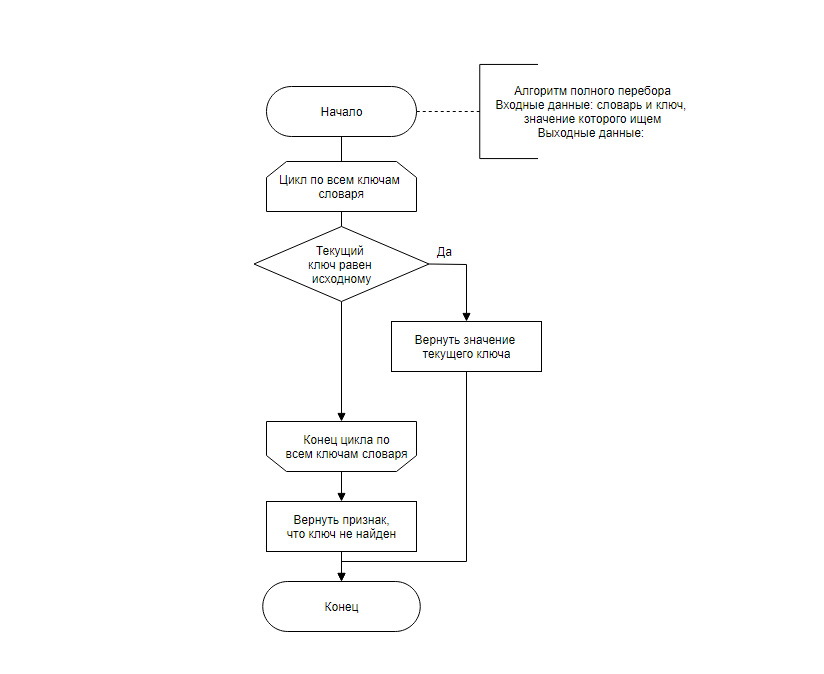
\includegraphics[width=1\linewidth]{assets/graphs/full_comb.png}
	\caption{Схема плотностного алгоритма DBSCAN}
	\label{fig:alg}
\end{figure}

\newpage
\section*{Вывод}

Была разработана схема алгоритма, необходимая для решения задачи.